\section{Experiments \& Empirical Analysis}
\label{sec:experiments}

\subsection{Experiment Setup}
\label{sec: experiment-setup}

We evaluate 12 systems in total: seven cascade, two hybrid, and three S2S. Configuration details are provided in Appendix~\ref{app:models-configuration}. Under the clean (unperturbed) condition, systems are evaluated on all 213 scenarios with $k = 5$  trials per scenario. We additionally evaluate under three perturbation conditions: French-accented user speech, coffee shop background noise, and both combined. To maintain feasibility across 12 systems and 3 conditions, perturbed evaluations use a randomly sampled subset of 90 scenarios (30 per domain) with $k = 3$ trials per scenario; the same subset is used across all systems. GPT-Realtime and Gemini Live models are evaluated using their native SDK \cite{google2024liveapi, openai2024realtimeapi}, \scribefull~+ \geminiflashfull~+ \conversationalfull~is evaluated using ElevenAgents \cite{elevenlabs2024agents}, and the remaining systems are evaluated using Pipecat \cite{pipecat2024}. All systems are evaluated using the respective framework's default turn detection configuration.


\subsection{Evaluation Reliability}
\label{sec: evaluation-reliability}

\framework~scores reflect genuine differences in agent behavior rather than evaluation artifacts: judge stochasticity contributes minimally to observed variance, and score differences between systems exceed measurement noise. We substantiate this with two sets of analyses: human-judge agreement to establish judge validity, and variance decomposition to complement bootstrap confidence intervals (CIs) in characterizing and bounding relative measurement noise.

\textbf{Human-Judge Agreement}
We measure inter-annotator agreement (IAA) between the judge and/or human annotators using quadratic-weighted Cohen's $\kappa$. Our reference baseline is the IAA of two independent annotations from linguist labellers (IAA-L). For judge inter-annotator agreement (IAA-J), each human annotation is paired with the judge score and pooled, with 95\% bootstrap confidence intervals (10{,}000 resamples) computed at the conversation level. \textbf{The judge meets the practical human IAA ceiling on all four metrics}, with IAA-J $\kappa$ ranging from 0.777 to 0.845 across metrics. For every metric, Spearman's $\rho$ and $\kappa$ (both computed on the same judge–human ratings) differ by at most 0.008, supporting the absence of systematic calibration bias. Full scores, details, and confidence intervals shown in \autoref{tab:judge-agreement}. 

\textbf{Variance Decomposition} Observed metric scores for a given model within a domain reflect variance from three sources: scenario difficulty, trial stochasticity (conversation trajectories), and LLM judge stochasticity. We characterize the contribution of each source on a subset of cascade and S2S models through complementary analyses, demonstrating that our main findings reflect genuine differences in model behaviour rather than measurement noise. Trial stochasticity was the dominant source of variance across all metrics and models, consistently exceeding scenario-level variance; judge stochasticity was minimal by comparison (permutation test, $p < 0.0001$ for all 16 model $\times$ metric combinations). For scenario variance, task completion and faithfulness showed the highest sensitivity, consistent with their observed dependence on intrinsic scenario difficulty and policy complexity. We also found that scenario difficulty rank is not shared uniformly across models but reflects model-specific response patterns (two-way random effects ICC, model $\times$ scenario interaction $p < 0.01$ and 4-18\% of total variance across evaluated domain $\times$ metric combinations). Full variance decomposition results are reported in Appendix~\ref{app:statistics}.

\subsection{Main Findings}
\label{sec:main-results}
\begin{figure}[t]
    \centering
    \captionsetup{font=small}
    \subfloat[\passatone]
    {{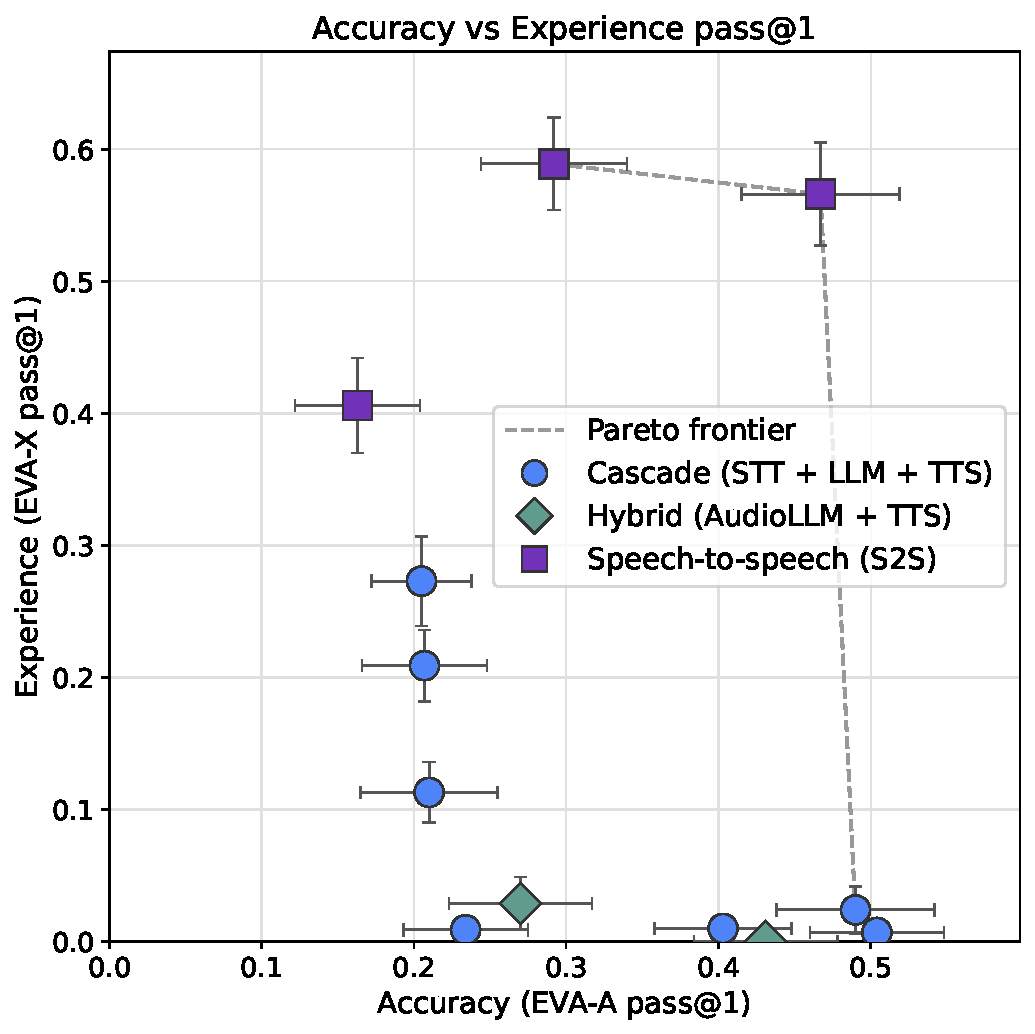
\includegraphics[width=.45\textwidth, trim=0pt 5pt 0pt 21pt, clip]{figures/accuracy_experience_plot/v6_accuracy_vs_experience_pass_at_1.pdf} }}%
    \qquad
    \subfloat[\passpowerk]
 {{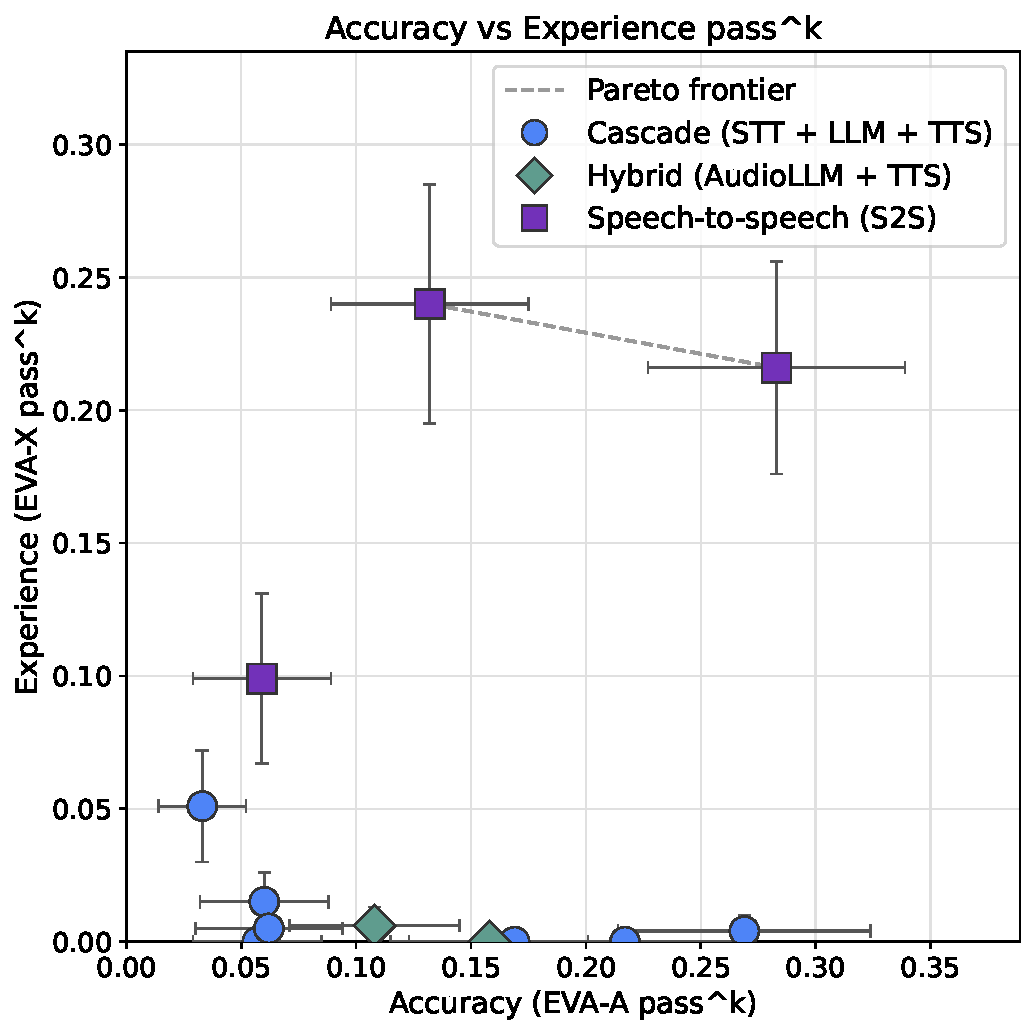
\includegraphics[width=.45\textwidth, trim=0pt 5pt 0 21pt, clip]{figures/accuracy_experience_plot/v6_accuracy_vs_experience_pass_power_k.pdf} }}%
    \captionsetup{font=small}
    \caption{\textbf{Accuracy vs Experience overview}. Accuracy and Experience scores for \passatone~and \passpowerk~, mean $\pm$ 95\% CIs across domains. On the \passatone~plot, four systems are on the Pareto frontier, two S2S and two cascade: \geminilive, \gptrealtime, \scribe~+ \geminiflash~+ \conversational, and \nova~+ \gpt~+ \sonic~(left to right). On the \passpowerk~plot, only the two S2S systems are on the frontier (note axis range differences).}
    \label{fig:accuracy-vs-experience}
\end{figure}


% Auto-generated by analysis/eva-bench-stats/run_paper.py
% Requires: xcolor, colortbl, booktabs, multirow, array
\definecolor{acc1}{HTML}{edeaf4}
\definecolor{acc2}{HTML}{d9d2e6}
\definecolor{acc3}{HTML}{bfb3d4}
\definecolor{acc4}{HTML}{9d8dbb}
\definecolor{acc5}{HTML}{7a679f}
\definecolor{acc6}{HTML}{584981}
\definecolor{acc7}{HTML}{3b3060}
\definecolor{tel1}{HTML}{b8dede}
\definecolor{tel2}{HTML}{90cece}
\definecolor{tel3}{HTML}{62b8b8}
\definecolor{tel4}{HTML}{3a9e9e}
\definecolor{tel5}{HTML}{1e8484}
\definecolor{tel6}{HTML}{0f6b6b}
\definecolor{tel7}{HTML}{075656}

% Auto-generated by analysis/eva-bench-stats/run_paper.py
% Requires: xcolor, colortbl, booktabs, multirow, array
\definecolor{acc1}{HTML}{edeaf4}
\definecolor{acc2}{HTML}{d9d2e6}
\definecolor{acc3}{HTML}{bfb3d4}
\definecolor{acc4}{HTML}{9d8dbb}
\definecolor{acc5}{HTML}{7a679f}
\definecolor{acc6}{HTML}{584981}
\definecolor{acc7}{HTML}{3b3060}
\definecolor{pnk1}{HTML}{fde4ec}
\definecolor{pnk2}{HTML}{fac4d4}
\definecolor{pnk3}{HTML}{f59ab5}
\definecolor{pnk4}{HTML}{ed6f95}
\definecolor{pnk5}{HTML}{db4577}
\definecolor{pnk6}{HTML}{b82d5c}
\definecolor{pnk7}{HTML}{8c1f44}

\begin{table}[h]
\centering\small
\captionsetup{font=small}
\caption{\textbf{Accuracy and Experience metrics} for all evaluated systems under clean-audio conditions, pooled equal-weighted across the three EVA domains. Each cell shows the pooled point estimate $\pm$ the percentile bootstrap CI half-width ($\alpha = 0.05$). The three pass-rate columns share a single shading scale so they can be visually compared; each submetric column is scaled independently. Darker = higher point estimate.}
\label{accuracy-experience-tables}
\resizebox{\textwidth}{!}{%
\begin{tabular}{ll@{\hskip 8pt}>{\centering\arraybackslash}p{1.8cm}@{\hskip 4pt}!{\color{white}\vrule width 0pt}@{\hskip 4pt}>{\centering\arraybackslash}p{1.8cm}@{\hskip 4pt}!{\color{white}\vrule width 0pt}@{\hskip 4pt}>{\centering\arraybackslash}p{1.8cm}@{\hskip 8pt}!{\color{black!25}\vrule}@{\hskip 8pt}>{\centering\arraybackslash}p{1.8cm}@{\hskip 8pt}!{\color{black!25}\vrule}@{\hskip 8pt}>{\centering\arraybackslash}p{1.8cm}@{\hskip 8pt}!{\color{black!25}\vrule}@{\hskip 8pt}>{\centering\arraybackslash}p{1.8cm}}
\toprule
 &  & \multicolumn{3}{c}{\textbf{EVA-A}} & \textbf{Task Completion} & \textbf{Faithfulness} & \textbf{Speech Fidelity} \\
\cmidrule{3-5} \cmidrule{6-6} \cmidrule{7-7} \cmidrule{8-8}
\textbf{Arch.} & \textbf{System} & \textbf{\passatone} & \textbf{\passatk} & \textbf{\passpowerk} & \textbf{Mean} & \textbf{Mean} & \textbf{Mean} \\
\midrule
\multirow{7}{*}{Cascade} & \cohere~+ \gemmaA~+ \voxtral & \cellcolor{acc2}\textcolor{black}{0.207 {\scriptsize $\pm$0.041}} & \cellcolor{acc4}\textcolor{white}{0.416 {\scriptsize $\pm$0.070}} & \cellcolor{acc1}\textcolor{black}{0.060 {\scriptsize $\pm$0.028}} & \cellcolor{tel1}\textcolor{black}{0.338 {\scriptsize $\pm$0.049}} & \cellcolor{tel3}\textcolor{black}{0.375 {\scriptsize $\pm$0.036}} & \cellcolor{tel6}\textcolor{white}{0.983 {\scriptsize $\pm$0.003}} \\
 & \scribe~+ \geminiflash~+ \conversational & \cellcolor{acc5}\textcolor{white}{0.490 {\scriptsize $\pm$0.052}} & \cellcolor{acc7}\textcolor{white}{0.730 {\scriptsize $\pm$0.058}} & \cellcolor{acc3}\textcolor{black}{0.269 {\scriptsize $\pm$0.055}} & \cellcolor{tel7}\textcolor{white}{0.736 {\scriptsize $\pm$0.043}} & \cellcolor{tel4}\textcolor{white}{0.457 {\scriptsize $\pm$0.042}} & \cellcolor{tel6}\textcolor{white}{0.977 {\scriptsize $\pm$0.006}} \\
 & \inkfull~+ \haikufull~+ \sonicfull & \cellcolor{acc2}\textcolor{black}{0.234 {\scriptsize $\pm$0.041}} & \cellcolor{acc5}\textcolor{white}{0.516 {\scriptsize $\pm$0.069}} & \cellcolor{acc1}\textcolor{black}{0.057 {\scriptsize $\pm$0.028}} & \cellcolor{tel1}\textcolor{black}{0.374 {\scriptsize $\pm$0.044}} & \cellcolor{tel5}\textcolor{white}{0.518 {\scriptsize $\pm$0.033}} & \cellcolor{tel6}\textcolor{white}{0.983 {\scriptsize $\pm$0.003}} \\
 & \novafull~+ \gptfull~+ \sonicfull & \cellcolor{acc5}\textcolor{white}{0.504 {\scriptsize $\pm$0.044}} & \cellcolor{acc7}\textcolor{white}{0.809 {\scriptsize $\pm$0.048}} & \cellcolor{acc2}\textcolor{black}{0.217 {\scriptsize $\pm$0.048}} & \cellcolor{tel5}\textcolor{white}{0.609 {\scriptsize $\pm$0.043}} & \cellcolor{tel7}\textcolor{white}{0.754 {\scriptsize $\pm$0.027}} & \cellcolor{tel7}\textcolor{white}{0.989 {\scriptsize $\pm$0.003}} \\
 & \novafull~+ \gptminifull~+ \aurafull & \cellcolor{acc2}\textcolor{black}{0.210 {\scriptsize $\pm$0.045}} & \cellcolor{acc4}\textcolor{white}{0.448 {\scriptsize $\pm$0.069}} & \cellcolor{acc1}\textcolor{black}{0.062 {\scriptsize $\pm$0.032}} & \cellcolor{tel3}\textcolor{black}{0.465 {\scriptsize $\pm$0.050}} & \cellcolor{tel2}\textcolor{black}{0.270 {\scriptsize $\pm$0.033}} & \cellcolor{tel6}\textcolor{white}{0.974 {\scriptsize $\pm$0.005}} \\
 & \parakeetfull~+ \gemmaBfull~+ \kokorofull & \cellcolor{acc4}\textcolor{white}{0.403 {\scriptsize $\pm$0.045}} & \cellcolor{acc7}\textcolor{white}{0.748 {\scriptsize $\pm$0.055}} & \cellcolor{acc2}\textcolor{black}{0.169 {\scriptsize $\pm$0.046}} & \cellcolor{tel6}\textcolor{white}{0.637 {\scriptsize $\pm$0.051}} & \cellcolor{tel4}\textcolor{white}{0.466 {\scriptsize $\pm$0.035}} & \cellcolor{tel4}\textcolor{white}{0.954 {\scriptsize $\pm$0.009}} \\
 & \whisper~+ \qwen~+ \voxtral & \cellcolor{acc2}\textcolor{black}{0.205 {\scriptsize $\pm$0.033}} & \cellcolor{acc5}\textcolor{white}{0.518 {\scriptsize $\pm$0.066}} & \cellcolor{acc1}\textcolor{black}{0.033 {\scriptsize $\pm$0.019}} & \cellcolor{tel2}\textcolor{black}{0.417 {\scriptsize $\pm$0.051}} & \cellcolor{tel5}\textcolor{white}{0.546 {\scriptsize $\pm$0.033}} & \cellcolor{tel1}\textcolor{black}{0.913 {\scriptsize $\pm$0.010}} \\
\midrule
\multirow{2}{*}{Hybrid} & \geminiflashfull~+ \geminiflashttsfull & \cellcolor{acc4}\textcolor{white}{0.431 {\scriptsize $\pm$0.047}} & \cellcolor{acc7}\textcolor{white}{0.812 {\scriptsize $\pm$0.055}} & \cellcolor{acc2}\textcolor{black}{0.158 {\scriptsize $\pm$0.043}} & \cellcolor{tel6}\textcolor{white}{0.674 {\scriptsize $\pm$0.041}} & \cellcolor{tel4}\textcolor{white}{0.443 {\scriptsize $\pm$0.036}} & \cellcolor{tel5}\textcolor{white}{0.969 {\scriptsize $\pm$0.006}} \\
 & \ultravoxfull & \cellcolor{acc3}\textcolor{black}{0.270 {\scriptsize $\pm$0.047}} & \cellcolor{acc5}\textcolor{white}{0.503 {\scriptsize $\pm$0.072}} & \cellcolor{acc1}\textcolor{black}{0.108 {\scriptsize $\pm$0.037}} & \cellcolor{tel3}\textcolor{black}{0.473 {\scriptsize $\pm$0.055}} & \cellcolor{tel2}\textcolor{black}{0.292 {\scriptsize $\pm$0.035}} & \cellcolor{tel5}\textcolor{white}{0.971 {\scriptsize $\pm$0.007}} \\
\midrule
\multirow{3}{*}{S2S} & \geminilivefull & \cellcolor{acc3}\textcolor{black}{0.292 {\scriptsize $\pm$0.048}} & \cellcolor{acc5}\textcolor{white}{0.552 {\scriptsize $\pm$0.069}} & \cellcolor{acc1}\textcolor{black}{0.132 {\scriptsize $\pm$0.043}} & \cellcolor{tel3}\textcolor{black}{0.473 {\scriptsize $\pm$0.052}} & \cellcolor{tel2}\textcolor{black}{0.238 {\scriptsize $\pm$0.035}} & \cellcolor{tel7}\textcolor{white}{0.995 {\scriptsize $\pm$0.003}} \\
 & \gptrealtimefull & \cellcolor{acc4}\textcolor{white}{0.467 {\scriptsize $\pm$0.052}} & \cellcolor{acc7}\textcolor{white}{0.710 {\scriptsize $\pm$0.061}} & \cellcolor{acc3}\textcolor{black}{0.283 {\scriptsize $\pm$0.056}} & \cellcolor{tel7}\textcolor{white}{0.739 {\scriptsize $\pm$0.046}} & \cellcolor{tel3}\textcolor{black}{0.360 {\scriptsize $\pm$0.041}} & \cellcolor{tel7}\textcolor{white}{0.996 {\scriptsize $\pm$0.002}} \\
 & \gptrealtimeminifull & \cellcolor{acc2}\textcolor{black}{0.163 {\scriptsize $\pm$0.041}} & \cellcolor{acc3}\textcolor{black}{0.318 {\scriptsize $\pm$0.063}} & \cellcolor{acc1}\textcolor{black}{0.059 {\scriptsize $\pm$0.030}} & \cellcolor{tel1}\textcolor{black}{0.345 {\scriptsize $\pm$0.054}} & \cellcolor{tel1}\textcolor{black}{0.125 {\scriptsize $\pm$0.031}} & \cellcolor{tel6}\textcolor{white}{0.977 {\scriptsize $\pm$0.012}} \\
\bottomrule
\end{tabular}%
}
\vspace{6pt}
\centering\small
\resizebox{\textwidth}{!}{%
\begin{tabular}{ll@{\hskip 8pt}>{\centering\arraybackslash}p{1.8cm}@{\hskip 4pt}!{\color{white}\vrule width 0pt}@{\hskip 4pt}>{\centering\arraybackslash}p{1.8cm}@{\hskip 4pt}!{\color{white}\vrule width 0pt}@{\hskip 4pt}>{\centering\arraybackslash}p{1.8cm}@{\hskip 8pt}!{\color{black!25}\vrule}@{\hskip 8pt}>{\centering\arraybackslash}p{1.8cm}@{\hskip 8pt}!{\color{black!25}\vrule}@{\hskip 8pt}>{\centering\arraybackslash}p{1.8cm}@{\hskip 8pt}!{\color{black!25}\vrule}@{\hskip 8pt}>{\centering\arraybackslash}p{1.8cm}}
% \toprule
 &  & \multicolumn{3}{c}{\textbf{EVA-X}} & \textbf{Turn-Taking} & \textbf{Conciseness} & \textbf{Conv. Progression} \\
\cmidrule{3-5} \cmidrule{6-6} \cmidrule{7-7} \cmidrule{8-8}
\textbf{Arch.} & \textbf{System} & \textbf{\passatone} & \textbf{\passatk} & \textbf{\passpowerk} & \textbf{Mean} & \textbf{Mean} & \textbf{Mean} \\
\midrule
\multirow{7}{*}{Cascade} & \cohere~+ \gemmaA~+ \voxtral & \cellcolor{acc2}\textcolor{black}{0.209 {\scriptsize $\pm$0.027}} & \cellcolor{acc5}\textcolor{white}{0.647 {\scriptsize $\pm$0.069}} & \cellcolor{acc1}\textcolor{black}{0.015 {\scriptsize $\pm$0.011}} & \cellcolor{pnk5}\textcolor{white}{0.567 {\scriptsize $\pm$0.024}} & \cellcolor{pnk6}\textcolor{white}{0.809 {\scriptsize $\pm$0.007}} & \cellcolor{pnk4}\textcolor{white}{0.598 {\scriptsize $\pm$0.032}} \\
 & \scribe~+ \geminiflash~+ \conversational & \cellcolor{acc1}\textcolor{black}{0.024 {\scriptsize $\pm$0.018}} & \cellcolor{acc1}\textcolor{black}{0.061 {\scriptsize $\pm$0.035}} & \cellcolor{acc1}\textcolor{black}{0.004 {\scriptsize $\pm$0.006}} & \cellcolor{pnk4}\textcolor{white}{0.451 {\scriptsize $\pm$0.019}} & \cellcolor{pnk5}\textcolor{white}{0.774 {\scriptsize $\pm$0.007}} & \cellcolor{pnk7}\textcolor{white}{0.804 {\scriptsize $\pm$0.023}} \\
 & \inkfull~+ \haikufull~+ \sonicfull & \cellcolor{acc1}\textcolor{black}{0.009 {\scriptsize $\pm$0.006}} & \cellcolor{acc1}\textcolor{black}{0.042 {\scriptsize $\pm$0.031}} & \cellcolor{acc1}\textcolor{black}{0.000 {\scriptsize $\pm$0.000}} & \cellcolor{pnk3}\textcolor{black}{0.312 {\scriptsize $\pm$0.020}} & \cellcolor{pnk5}\textcolor{white}{0.784 {\scriptsize $\pm$0.007}} & \cellcolor{pnk6}\textcolor{white}{0.710 {\scriptsize $\pm$0.023}} \\
 & \novafull~+ \gptfull~+ \sonicfull & \cellcolor{acc1}\textcolor{black}{0.007 {\scriptsize $\pm$0.006}} & \cellcolor{acc1}\textcolor{black}{0.031 {\scriptsize $\pm$0.024}} & \cellcolor{acc1}\textcolor{black}{0.000 {\scriptsize $\pm$0.000}} & \cellcolor{pnk3}\textcolor{black}{0.283 {\scriptsize $\pm$0.019}} & \cellcolor{pnk7}\textcolor{white}{0.835 {\scriptsize $\pm$0.007}} & \cellcolor{pnk6}\textcolor{white}{0.737 {\scriptsize $\pm$0.020}} \\
 & \novafull~+ \gptminifull~+ \aurafull & \cellcolor{acc1}\textcolor{black}{0.113 {\scriptsize $\pm$0.023}} & \cellcolor{acc3}\textcolor{black}{0.416 {\scriptsize $\pm$0.070}} & \cellcolor{acc1}\textcolor{black}{0.005 {\scriptsize $\pm$0.004}} & \cellcolor{pnk5}\textcolor{white}{0.583 {\scriptsize $\pm$0.019}} & \cellcolor{pnk7}\textcolor{white}{0.835 {\scriptsize $\pm$0.008}} & \cellcolor{pnk1}\textcolor{black}{0.428 {\scriptsize $\pm$0.025}} \\
 & \parakeetfull~+ \gemmaBfull~+ \kokorofull & \cellcolor{acc1}\textcolor{black}{0.010 {\scriptsize $\pm$0.009}} & \cellcolor{acc1}\textcolor{black}{0.035 {\scriptsize $\pm$0.032}} & \cellcolor{acc1}\textcolor{black}{0.000 {\scriptsize $\pm$0.000}} & \cellcolor{pnk3}\textcolor{black}{0.308 {\scriptsize $\pm$0.015}} & \cellcolor{pnk7}\textcolor{white}{0.829 {\scriptsize $\pm$0.007}} & \cellcolor{pnk7}\textcolor{white}{0.774 {\scriptsize $\pm$0.024}} \\
 & \whisper~+ \qwen~+ \voxtral & \cellcolor{acc2}\textcolor{black}{0.273 {\scriptsize $\pm$0.034}} & \cellcolor{acc5}\textcolor{white}{0.684 {\scriptsize $\pm$0.065}} & \cellcolor{acc1}\textcolor{black}{0.051 {\scriptsize $\pm$0.021}} & \cellcolor{pnk5}\textcolor{white}{0.561 {\scriptsize $\pm$0.029}} & \cellcolor{pnk1}\textcolor{black}{0.685 {\scriptsize $\pm$0.010}} & \cellcolor{pnk4}\textcolor{white}{0.612 {\scriptsize $\pm$0.026}} \\
\midrule
\multirow{2}{*}{Hybrid} & \geminiflashfull~+ \geminiflashttsfull & \cellcolor{acc1}\textcolor{black}{0.000 {\scriptsize $\pm$0.000}} & \cellcolor{acc1}\textcolor{black}{0.000 {\scriptsize $\pm$0.000}} & \cellcolor{acc1}\textcolor{black}{0.000 {\scriptsize $\pm$0.000}} & \cellcolor{pnk1}\textcolor{black}{0.019 {\scriptsize $\pm$0.003}} & \cellcolor{pnk6}\textcolor{white}{0.801 {\scriptsize $\pm$0.007}} & \cellcolor{pnk4}\textcolor{white}{0.618 {\scriptsize $\pm$0.029}} \\
 & \ultravoxfull & \cellcolor{acc1}\textcolor{black}{0.029 {\scriptsize $\pm$0.020}} & \cellcolor{acc1}\textcolor{black}{0.081 {\scriptsize $\pm$0.039}} & \cellcolor{acc1}\textcolor{black}{0.006 {\scriptsize $\pm$0.007}} & \cellcolor{pnk4}\textcolor{white}{0.417 {\scriptsize $\pm$0.020}} & \cellcolor{pnk4}\textcolor{white}{0.750 {\scriptsize $\pm$0.010}} & \cellcolor{pnk1}\textcolor{black}{0.429 {\scriptsize $\pm$0.030}} \\
\midrule
\multirow{3}{*}{S2S} & \geminilivefull & \cellcolor{acc5}\textcolor{white}{0.589 {\scriptsize $\pm$0.035}} & \cellcolor{acc7}\textcolor{white}{0.979 {\scriptsize $\pm$0.021}} & \cellcolor{acc2}\textcolor{black}{0.240 {\scriptsize $\pm$0.045}} & \cellcolor{pnk7}\textcolor{white}{0.830 {\scriptsize $\pm$0.017}} & \cellcolor{pnk6}\textcolor{white}{0.801 {\scriptsize $\pm$0.009}} & \cellcolor{pnk5}\textcolor{white}{0.636 {\scriptsize $\pm$0.029}} \\
 & \gptrealtimefull & \cellcolor{acc5}\textcolor{white}{0.566 {\scriptsize $\pm$0.039}} & \cellcolor{acc7}\textcolor{white}{0.939 {\scriptsize $\pm$0.034}} & \cellcolor{acc2}\textcolor{black}{0.216 {\scriptsize $\pm$0.040}} & \cellcolor{pnk7}\textcolor{white}{0.815 {\scriptsize $\pm$0.013}} & \cellcolor{pnk6}\textcolor{white}{0.801 {\scriptsize $\pm$0.008}} & \cellcolor{pnk5}\textcolor{white}{0.679 {\scriptsize $\pm$0.024}} \\
 & \gptrealtimeminifull & \cellcolor{acc3}\textcolor{black}{0.406 {\scriptsize $\pm$0.036}} & \cellcolor{acc7}\textcolor{white}{0.893 {\scriptsize $\pm$0.043}} & \cellcolor{acc1}\textcolor{black}{0.099 {\scriptsize $\pm$0.032}} & \cellcolor{pnk7}\textcolor{white}{0.818 {\scriptsize $\pm$0.015}} & \cellcolor{pnk2}\textcolor{black}{0.722 {\scriptsize $\pm$0.009}} & \cellcolor{pnk1}\textcolor{black}{0.388 {\scriptsize $\pm$0.033}} \\
\bottomrule
\end{tabular}%
}
\end{table}


% Auto-generated by analysis/eva-bench-stats/paper_plot_perturbation.py
% Requires: graphicx, xcolor
\definecolor{pertaccent}{HTML}{00C49A}
\definecolor{pertbgnoise}{HTML}{F8E16C}
\definecolor{pertboth}{HTML}{156064}
\begin{figure}[t]
\centering
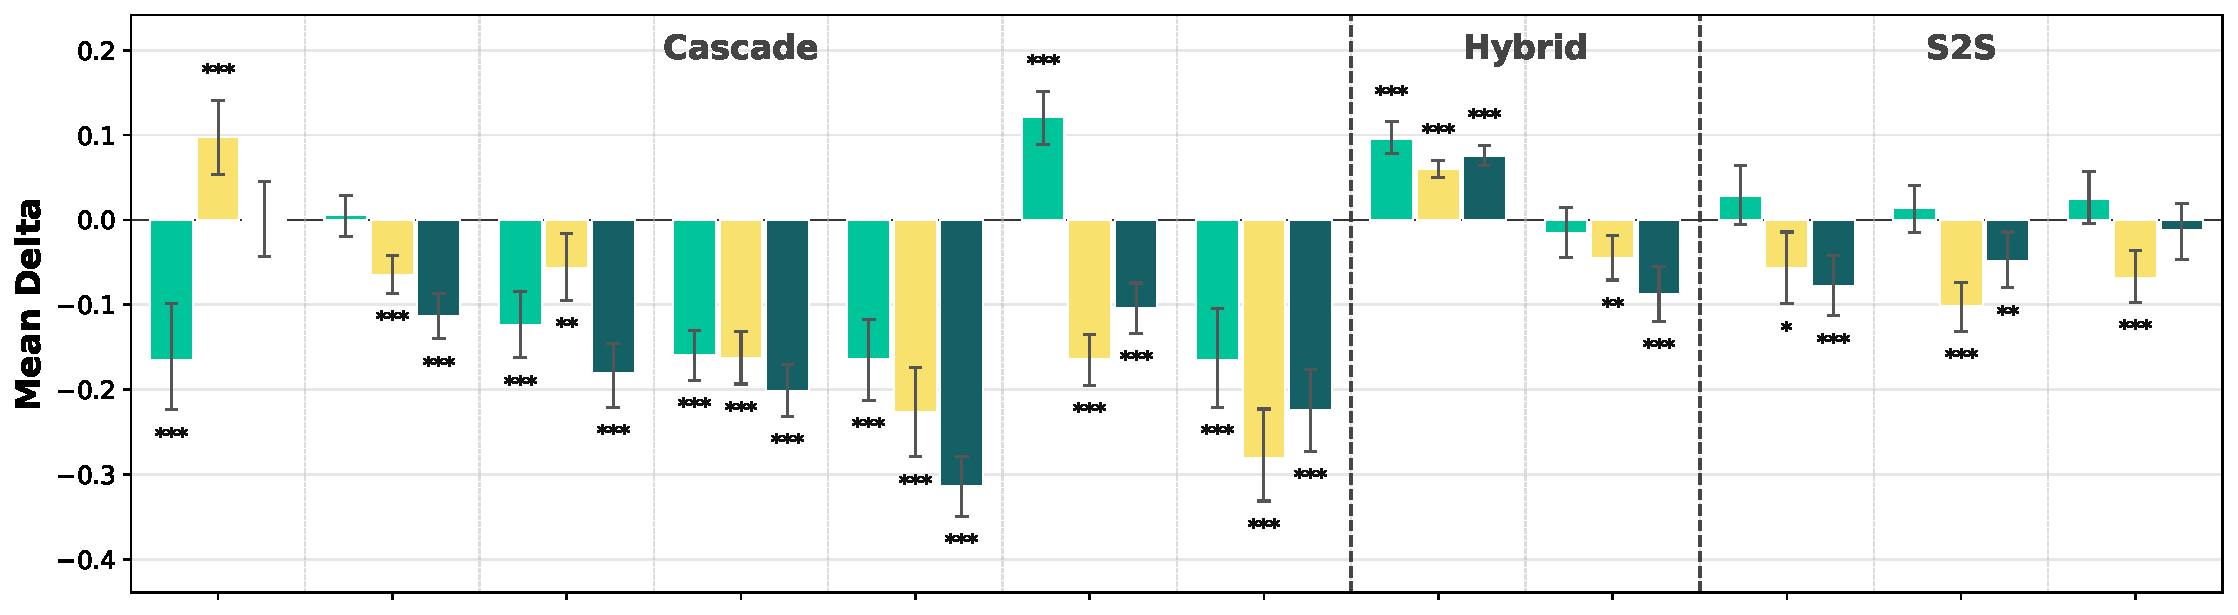
\includegraphics[width=\linewidth]{figures/perturbations/paper_turn_taking_perturbation_pooled.pdf}
\captionsetup{font=small}
\caption{Perturbation effect on  \textbf{\metricturntaking} pooled across domains. Bars show the mean delta from clean trials; 95\% bootstrap (CIs) on the per-scenario delta. Bar colors encode the perturbation condition: \textcolor{pertaccent}{$\blacksquare$}~accent, \textcolor{pertbgnoise}{$\blacksquare$}~background noise, \textcolor{pertboth}{$\blacksquare$}~accent~+~background noise. Asterisks mark cells significant after Holm-Bonferroni correction (\texttt{*}~$p<0.05$, \texttt{**}~$p<0.01$, \texttt{***}~$p<0.001$). Models listed in Appendix~\ref{app:perturbations}.}
\label{fig:perturbation-transcription-pooled-turn-taking-final}
\end{figure}


\textbf{Accuracy–Experience Frontier}

No evaluated system clears 0.5 on both EVA-A \passatone\ and EVA-X \passatone\ jointly, and only \gptrealtime~(0.47, 0.57) clears 0.4 on both. This sparsity is reflected in the \passatone\ Pareto frontier (Figure~\ref{fig:accuracy-vs-experience}a), which contains four systems spanning two disjoint regions.

Within EVA-X, the gap is almost entirely driven by \metricturntaking, where mean scores stratify cleanly by architecture (cascade: 0.28–0.58; S2S: 0.82–0.83) (Table~\ref{accuracy-experience-tables}). \metricconcise~and \metricconversationprogression~show no comparable separation. The two hybrid systems both fall within the cascade EVA-X range (0.000, 0.029), suggesting that hybrid systems may not inherit the latency advantages of fully speech-to-speech architectures, though more systems would be needed to confirm this.

Among the evaluated cascade systems, we observe a consistent accuracy–experience trade-off, pointing to a potential underlying capability–latency tension. The three cascade systems that perform best on accuracy (\nova~+ \gpt~+ \sonic, \scribe~+ \geminiflash~+ \conversational, \parakeet~+ \gemmaB~+ \kokoro) struggle on experience, with mean latencies on tool-call turns above 5\,s. In contrast, the two cascade systems with better experience (\whisper~+ \qwen~+ \voxtral, \cohere~+ \gemmaA~+ \voxtral) achieve tool-call turn latencies below 2.7\,s but also lower accuracy. No cascade system exceeds 0.25 on both dimensions, with no overlapping CIs. Full latency breakdowns appear in Table~\ref{tab:appendix-turntaking-response-speed}.

\textbf{Consistency Analysis}
Across all 12 evaluated systems, peak performance (\passatk) substantially exceeds reliable performance (\passpowerk) on both axes: the median gap is 0.44 on EVA-A and 0.24 on EVA-X. Under the \passpowerk~interpretation (the probability of passing all five trials on a given scenario) even the strongest systems fall well below peak, suggesting that single-trial scores systematically overstate deployment-grade reliability.

\textbf{Robustness Analysis.}
We evaluate each system under three perturbation conditions -- accented speech, background noise, and both combined -- measuring performance degradation against a clean baseline across the 90 subsampled scenarios (see \autoref{sec: experiment-setup}) via paired sign-flip permutation tests ($n{=}90$, Holm--Bonferroni corrected). The two architectures diverge in their failure modes: cascade systems are most vulnerable on accuracy metrics, while S2S systems suffer most on experience metrics. Accented speech drives the largest accuracy failures: cascade task completion drops by a mean 10 points (worst system: 17 points), while no S2S model shows significant accuracy degradation (0/27 model-metric pairs). Background noise exposes S2S experience failures (EVA-X $\bar{\Delta}{=}{-}0.16$), though cascade accuracy also suffers under noise (task completion $\bar{\Delta}{=}{-}0.10$ vs.\ S2S $\bar{\Delta}{=}{-}0.04$). The combined condition reveals the full spread: cascade task completion drops a mean 19 points (worst systems: 31 points), while the S2S model mean remains within 5 points. 

Within the cascade class, however, robustness varies considerably, with as low as 11\% and as high as 87\% of per-system metric-perturbation combinations showing significant degradation. The two most robust cascade systems degrade primarily on experience metrics, more closely resembling S2S systems than their cascade peers. Turn-taking is the most perturbation-sensitive metric overall, with 81\% of measurements across perturbations and systems showing significant degradation. See \autoref{fig:perturbation-transcription-pooled-turn-taking-final} and Appendix~\ref{app:perturbations} for full results.

\subsection{Failure Mode Analysis}
\label{sec:failure-modes}
\framework's metrics enable detailed error analysis. We report four targeted analyses below, with additional analyses in Appendix~\ref{app:metrics-analysis}.



\textbf{Named entity transcription as an accuracy bottleneck.}
\framework's diagnostic metrics reveal a consistent association between \metrictranscription~and \metrictaskcompletion~across all three domains, pointing to transcription as a candidate bottleneck for cascade system performance. Across seven cascade systems, mean transcription accuracy on key entities is strongly correlated with mean task completion (Pearson $r =$ 0.93, $p =$ 0.002)  and the relationship holds within each domain ($r =$ 0.88–0.93, all $p <$ 0.01). Cascade systems with transcription accuracy below 70\% on key entities show task completion rates 39\% lower than systems above this threshold (0.37 vs 0.60), with a consistent drop in each domain (ITSM: $-41\%$, HR: $-41\%$, CSM: $-34\%$). See \autoref{fig:transcription_accuracy_task_completion} for the correlation plot and \autoref{fig:stt_transcription_accuracy} for \metrictranscription~scores.

\textbf{Evaluated S2S systems show contrasting patterns relative to other systems}. The higher EVA-X scores for S2S systems reflect a clear turn-taking lead with on-time rate and conversation completion up +27.9 pp and +15.2 pp on average respectively, though the strongest cascade systems come within a few percentage points. The conversation completion gap is partly explained by many cascade systems completely failing to respond to short utterances and spelled content. S2S systems also show policy adherence issues, violating stated policy more often on average (+24.6 pp) and trailing the strongest cascade systems on this aspect. Confidence intervals, per-system breakdowns, and additional details are in Appendix~\ref{app:pipeline-comparison}.

\textbf{Faithfulness failures are not predicted by task completion.}
$72.2\%$ of conversations ($n=12,780$) with task completion = 1 exhibit at least one faithfulness deviation (faithfulness < 1.0), indicating that agents frequently make policy deviations or hallucinate details even when they call the correct tools. Conversely, $50.5\%$ of faithfulness deviations co-occur with task completion = 0, suggesting that some task failures are downstream of faithfulness violations. This decoupling motivates including faithfulness as an independent metric. See Appendix~\ref{app:faith_tc} for full confusion matrix.

\textbf{Speech fidelity failures concentrate on alphanumeric entities.}
Entity errors (letter substitutions, digit omissions, spurious insertions, and phonetic confusions between similar-sounding characters) are the dominant speech fidelity failure mode across all evaluated models. This motivates including speech fidelity as an audio-level metric: a caller who receives a misarticulated confirmation code cannot detect the error from context alone, and even 1\% per-turn fail rates represent a non-trivial error probability over multi-turn interactions. See Appendix~\ref{app:speech-fidelity} for examples of failures.